To give credibility to the approach mentioned in Chapter 3, a simple test case to test the capabilities of HTM and confirm that they apply on a video is introduced.
\section{Bouncing Ball Test}

\begin{figure}[H]
\centering
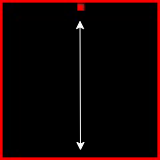
\includegraphics[width=.3\textwidth]{resources/experiments/bouncing_ball/bb_updown1.png}\hfill
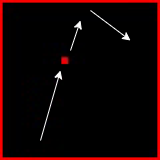
\includegraphics[width=.3\textwidth]{resources/experiments/bouncing_ball/bb_updownside.png}\hfill
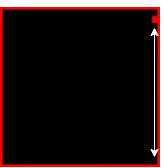
\includegraphics[width=.3\textwidth]{resources/experiments/bouncing_ball/bb_updown2.png}
\caption{The bouncing ball test}
\label{fig:bb}
\end{figure}
The video consists of a ball bouncing up and down until an anomaly occurs in the form of a sudden introduction of a horizontal velocity. After a while this horizontal velocity goes back to 0 and the ball goes back to bouncing up and down in-place.
\section{Surveillance example}